\documentclass[HARVARD,Utopia2COL]{WileyNJDv5}

\usepackage{amsmath,amssymb,booktabs}
\usepackage{graphicx}
\hypersetup{hidelinks}

\articletype{Research Article}
\journal{Journal of Futures Markets}
\raggedbottom

\begin{document}

\title{When Does Posterior Integration Change Option Values? Evidence from WTI Average Price Options}

\author[1]{Heriberto Espino Montelongo}
\authormark{ESPINO MONTELONGO}
\titlemark{POSTERIOR INTEGRATION IN WTI AVERAGE PRICE OPTIONS}

\address[1]{\orgname{Universidad de las Am\'ericas Puebla}, \orgaddress{\state{Puebla}, \country{Mexico}}}
\corres{Corresponding author: Heriberto Espino Montelongo. \email{[corresponding email]}}

\abstract[Abstract]{
This paper studies when parameter uncertainty materially changes an arithmetic-average option value and compares that effect with changing the volatility input itself. The posterior-integrated price (PI) averages the conditional risk-neutral option value over the volatility posterior, whereas the posterior-mean plug-in price (PM) evaluates that value at posterior mean volatility. Their difference is locally governed by posterior variance and the curvature of the option-pricing function. A 175,000-history synthetic experiment confirms this mechanism and identifies weak-information, high-curvature states in which the difference is economically meaningful. In the observed WTI Average Price Option sample, however, the mean absolute PI--PM difference is \$0.000745 per barrel while the mean width of the 95\% posterior interval for the model price is \$0.2733 per barrel. Thus a small effect on the posterior mean price does not imply little parameter uncertainty in option values. In 2,381 out-of-sample contract-date observations, prior option-implied volatility inputs produce much lower pricing errors than the historical-volatility benchmarks evaluated here. The result is robust to rolling-window, EWMA, and horizon-matched GARCH comparisons, does not require a flexible implied-volatility smile, and persists in a cross-instrument validation using vanilla-WTI options.
}

\keywords{Bayesian option pricing; Asian options; WTI crude oil; parameter uncertainty; implied volatility}

\maketitle

\section{Introduction}\label{sec:short_intro}

Option prices depend on parameters that are estimated rather than observed. A Bayesian analysis can account for this uncertainty by integrating the conditional option value over the posterior distribution instead of fixing all parameters at point estimates. This idea is established in Bayesian option pricing and forecasting \citep{guidolin2003,romboutsstentoft2014,guptareisinger2014}. The practical question is narrower: when does that integration materially change the option value?

Arithmetic-average Asian options provide a useful setting because their exposure to volatility changes with moneyness, maturity, and the fraction of the averaging period already fixed. The numerical literature has developed efficient methods for this path dependence, including geometric-average control variates and conditioning approximations \citep{kemnavorst1990,curran1994}. Commodity applications additionally require a term structure of futures prices and, in richer specifications, stochastic convenience yields, jumps, or stochastic volatility \citep{schwartz1997,shirayatakahashi2011,ewaldwu2023}. The objective here is not to introduce another Asian-option model. It is to isolate the effect of parameter uncertainty within a transparent pricing model and to compare that effect with the empirical importance of the volatility information supplied to the model.

The distinction matters because two different questions are easily conflated. The first is whether averaging the conditional option value over a posterior distribution changes the point estimate relative to a posterior-mean plug-in price. The second is whether the volatility input itself is aligned with the volatility information embedded in option prices. These are conceptually separate. The first is a nonlinear-averaging problem. The second concerns model specification and information content.

Let \(C^Q(\sigma)\) be the risk-neutral option value conditional on volatility \(\sigma\), let \(\mathcal D\) denote the historical return data, and let \(\bar\sigma=\mathbb E[\sigma\mid\mathcal D]\). The posterior-integrated price and posterior-mean plug-in price are
\begin{equation}
 C_{PI}=\mathbb E[C^Q(\sigma)\mid\mathcal D],
 \qquad
 C_{PM}=C^Q(\bar\sigma).
 \label{eq:short_pi_pm}
\end{equation}
A second-order expansion gives
\begin{equation}
 C_{PI}-C_{PM}
 \approx
 \frac12 C^{Q\prime\prime}(\bar\sigma)
 \operatorname{Var}(\sigma\mid\mathcal D).
 \label{eq:short_taylor}
\end{equation}
Posterior integration therefore matters when parameter uncertainty coincides with curvature of the option-pricing function. By contrast, the dispersion of the posterior distribution of model prices is locally first order in the posterior standard deviation. A small PI--PM difference need not imply little uncertainty in the theoretical option value.

The empirical application uses WTI Average Price Options (APOs), whose payoff depends on the arithmetic average of daily first-nearby WTI futures settlements. WTI is useful for this comparison because historical volatility can change sharply, the futures curve varies across valuation dates, and option-implied volatility is observable from both the APO market and a separate vanilla-WTI option market. The information cutoff is asymmetric by construction: option-implied volatility inputs use only option observations from dates strictly earlier than the target date, while repricing conditions on the target-date futures curve, realized fixings, and discount factor. Historical-volatility estimators use returns available under their stated valuation-date cutoff.

Three findings organize the paper. First, a large synthetic experiment confirms Equation~\eqref{eq:short_taylor}: posterior integration becomes important primarily in weak-information states with substantial volatility curvature and little of the averaging period already fixed. Second, the observed October-2026 WTI sample lies in a region where posterior-integrated and posterior-mean plug-in prices are almost identical, even though the posterior distribution of model prices remains materially dispersed. Third, prior option-implied volatility inputs produce substantially lower out-of-sample pricing errors than the historical-volatility benchmarks evaluated here. Rolling historical windows, EWMA, and a horizon-matched GARCH(1,1) forecast do not reproduce that performance. A same-contract lagged-IV benchmark shows that the result does not require a flexible cross-sectional smile, and a separate validation using vanilla-WTI options shows that it is not confined to volatility inferred from the APO family itself.

These results do not identify a pure structural difference between physical and risk-neutral volatility. Implied volatility under a parsimonious pricing model can absorb risk premia, stochastic volatility, jumps, omitted futures-curve dynamics, liquidity, and settlement conventions. The supported statement is therefore empirical and conditional: in this sample, prior option-implied volatility contains substantially more information for subsequent APO settlement pricing than the historical-volatility inputs considered here, while posterior integration of the historical-volatility distribution changes the point-price mean much less.

The remainder of the paper is organized around those three findings. Section~\ref{sec:short_method} develops the posterior-pricing mechanism. Section~\ref{sec:short_design} describes the WTI data and out-of-sample design. Section~\ref{sec:short_results} reports the synthetic and empirical results. Section~\ref{sec:short_robustness} summarizes robustness and interpretation, with complete historical-benchmark, numerical, liquidity, and external-transfer diagnostics reported in Online Supplement Sections S1--S4. Section~\ref{sec:short_conclusion} concludes.

\section{Posterior uncertainty and Asian-option pricing}\label{sec:short_method}

\subsection{Physical inference and risk-neutral valuation}

Historical log returns are modeled under the physical measure as
\begin{equation}
 R_i\sim
 \mathcal N\!\left[
 \left(\mu-\frac12\sigma^2\right)\Delta t,
 \sigma^2\Delta t
 \right],
 \label{eq:short_returns}
\end{equation}
with baseline priors
\begin{equation}
 \mu\sim\mathcal N(0,1),
 \qquad
 \sigma\sim\operatorname{InvGamma}(2,0.1),
 \qquad \sigma>0.
 \label{eq:short_priors}
\end{equation}
The empirical posterior is sampled in \((\mu,\log\sigma)\) with a random-walk Metropolis algorithm. For the large synthetic experiment, \(\mu\) is integrated analytically conditional on \(\sigma\), leaving a one-dimensional posterior calculation. This removes MCMC error from the mechanism experiment without changing the statistical model.

Pricing is carried out separately under the risk-neutral measure. For futures maturity \(u\), the maintained benchmark is
\begin{equation}
 dF_t^u=\sigma F_t^u\,dW_t^Q,
 \label{eq:short_q}
\end{equation}
where \(u\) indexes futures maturity and the same Brownian motion \(W^Q\) drives all maturities. This common-factor assumption fixes the cross-maturity dependence relevant for the variance of the arithmetic average. The historical drift does not enter the option value. The constant-volatility, one-factor specification is intentionally parsimonious: it provides a common pricing model within which the effect of posterior integration and the effect of changing the volatility input can be compared directly.

For an arithmetic-average option with fixing dates \(t_1,\ldots,t_M\),
\begin{equation}
 A_T=\frac{1}{M}\sum_{j=1}^M F^{(1)}_{t_j},
 \label{eq:short_average}
\end{equation}
and the conditional call value is
\begin{equation}
 C_t^Q(\sigma)
 =
 B(t,T)\,
 \mathbb E^Q\!\left[
 (A_T-K)^+\mid\mathcal F_t;\sigma
 \right],
 \label{eq:short_call_value}
\end{equation}
where \(B(t,T)\) is the discount factor, \(K\) the strike, and \(\mathcal F_t\) the valuation-date information set. Put values are defined analogously.
where \(F^{(1)}_{t_j}\) is the first-nearby WTI futures settlement applicable to fixing date \(t_j\). At a valuation date inside the averaging period, already realized fixings enter \(A_T\) deterministically and only the remaining fixings are stochastic. Each remaining fixing is initialized from the corresponding point of the observed CL futures curve.

The baseline historical-volatility prices are evaluated by Monte Carlo. Curran's conditioning approximation \citep{curran1994} is used as a deterministic pricing approximation for the large out-of-sample comparisons and scalar-volatility sensitivity calculations. High-precision pseudo-random Monte Carlo and scrambled Sobol calculations are used only as numerical checks.

\subsection{Posterior integration and price uncertainty}

Equation~\eqref{eq:short_pi_pm} compares two summaries of the same posterior and the same pricing model. A Taylor expansion of \(C^Q(\sigma)\) around \(\bar\sigma\) yields Equation~\eqref{eq:short_taylor}. The leading PI--PM difference depends on two quantities: posterior variance and the curvature of the option-pricing function with respect to volatility. The correction can have either sign because the local curvature can be positive or negative. The second-order approximation is most accurate when the posterior is sufficiently concentrated and higher-order curvature is controlled over the relevant posterior support.

The posterior distribution also induces a distribution of theoretical option values,
\begin{equation}
 C^Q(\sigma),\qquad \sigma\sim p(\sigma\mid\mathcal D).
 \label{eq:short_pushforward}
\end{equation}
Its dispersion is approximately
\begin{equation}
 \operatorname{SD}\!\left(C^Q(\sigma)\mid\mathcal D\right)
 \approx
 \left|C^{Q\prime}(\bar\sigma)\right|
 \sqrt{\operatorname{Var}(\sigma\mid\mathcal D)}.
 \label{eq:short_delta}
\end{equation}
The contrast between Equations~\eqref{eq:short_taylor} and \eqref{eq:short_delta} is central. The change in the posterior mean price is locally second order in posterior dispersion, whereas uncertainty in the theoretical option value is locally first order. It is therefore possible for \(C_{PI}\) and \(C_{PM}\) to be almost identical while the posterior distribution of model prices remains economically nontrivial.

The paper uses the terms \emph{posterior-integrated price} and \emph{posterior-mean plug-in price} only for this comparison. The former is the posterior average of the conditional option value; the latter evaluates the same pricing model at posterior mean volatility. Neither is interpreted as a market-consistent price outside the maintained model.

\subsection{Synthetic mechanism experiment}

The synthetic experiment is designed to vary the two ingredients in Equation~\eqref{eq:short_taylor}. It contains 175,000 independently generated return histories across historical sample sizes from 21 to 1,260 observations and annual volatility levels from 0.10 to 0.80. The option layer varies maturity, moneyness, and the fraction of the arithmetic average already fixed. For each history and contract state, the experiment computes the actual PI--PM difference, posterior variance of volatility, local price curvature, and the second-order approximation.

The purpose is not to establish that posterior integration is always important or always negligible. It is to identify the regions of the state space in which the nonlinear averaging effect becomes economically meaningful and to determine whether Equation~\eqref{eq:short_taylor} explains those regions.

\section{Data and empirical design}\label{sec:short_design}

\subsection{WTI Average Price Options}

The empirical sample is built from individual Barchart histories for WTI Average Price Options. The raw archive contains 213 unique contracts and 11,179 option-date observations across expiries from September 2026 through June 2029. The market target is the Barchart end-of-day settlement field. Calls and puts are retained as available, and moneyness is recomputed by valuation date rather than assigned once at the contract level.

For each option-date observation, the pricing data reconstruct three objects: realized first-nearby CL settlements for fixing dates that have already occurred, the CL futures contracts applicable to the remaining fixing dates, and the contemporaneous futures term structure used to initialize those remaining fixings. This preserves the contract feature that the first-nearby futures contract can change during the averaging month.

Historical volatility is estimated from WTI futures returns available by the valuation date. The baseline uses the labelled continuous/front-month \texttt{CL=F} return series as the physical-measure proxy. A robustness check reconstructs a first-nearby return history contract by contract from CL settlements and excludes returns spanning contract switches.

\subsection{Out-of-sample volatility comparisons}

The main empirical experiment asks how different volatility inputs affect subsequent APO pricing. The timing convention separates volatility estimation from repricing information. Option-implied volatility inputs use only option observations dated strictly before the target date; target-date repricing uses the contemporaneous futures curve, realized fixings, and discount factor. Historical-volatility estimators use returns available under their stated valuation-date cutoff. Seven expiries pass the committed-data coverage requirement, producing 2,381 out-of-sample contract-date observations over 15 target dates.

The historical-volatility benchmark is the posterior-integrated price based on the expanding historical return sample. Four pre-specified recent historical alternatives use the most recent 63, 126, or 252 returns and an EWMA estimate with a 63-business-day half-life; complete results are reported in Online Supplement Section S1 and Table S1. A Gaussian GARCH(1,1) provides a stronger dynamic benchmark. For each target date, GARCH parameters are estimated only from earlier returns; the target-date return updates only the end-of-day conditional variance state, after which conditional variances are forecast across the remaining fixing horizon and collapsed to a constant annualized volatility that matches the implied variance of the unresolved arithmetic-average component under the maintained one-factor pricing model.

The option-implied specifications are also restricted to earlier dates. Contract-level APO implied volatilities are obtained by inverting the Curran pricing approximation. A previous-day smile uses the latest completed earlier APO date for the relevant expiry, while an expanding specification uses all earlier dates with recency weights. The fitted relation is a function of moneyness and option type. Same-day APO settlements never enter the target-date volatility estimate.

A separate persistence benchmark tests whether the improvement requires a fitted smile. For each contract with an earlier implied volatility observation, the latest strictly prior IV for that same contract is carried forward and the contract is repriced using the current futures curve, discount factor, realized fixings, and remaining fixing schedule. This comparison is available for 2,366 of the 2,381 observations.

Pricing performance is summarized by mean error, mean absolute error (MAE), and root mean squared error (RMSE). Dependence across contracts observed on the same valuation date is preserved with valuation-date cluster bootstrap resampling.

\subsection{Cross-instrument validation}

The APO experiment still obtains implied volatility from the same option family later used as the pricing target. An independent validation therefore uses standard monthly American WTI options on futures (CME product LO) obtained through Databento. Official LO option settlements are matched to CL futures settlements, and contract-level implied volatilities are recovered with a Cox--Ross--Rubinstein futures-option tree.

For each APO target date, only LO observations from earlier dates are used. Implied-volatility smiles are fitted separately for the underlying CL futures contracts needed by the October-2026 APO fixing schedule. The resulting maturity-specific volatilities are mapped into the maintained scalar-volatility APO pricing model. The main comparison is restricted to 253 APO contract-date observations, spanning 10 target dates, that lie within the observed prior LO moneyness support for both external specifications. Alternative scalar transfers and CRR tree-refinement diagnostics are reported in Online Supplement Section S4 and Table S4.

The cross-instrument experiment is not intended to estimate a structural variance risk premium. Its role is narrower: it asks whether the out-of-sample improvement associated with prior option-implied volatility remains when the volatility information comes from a separate WTI option market rather than from earlier APO settlements.

\section{Results}\label{sec:short_results}

\subsection{When does posterior integration matter?}

Figure~\ref{fig:short_mechanism} summarizes the synthetic mechanism experiment. The PI--PM difference grows when historical information is weak, volatility is high, maturity is long, little of the arithmetic average has already been fixed, and the option-pricing function is strongly curved in volatility. Across the full synthetic experiment, the maximum absolute PI--PM difference is 0.1384 on a normalized \$100 forward, and the largest cell-level 99th percentile is 0.1271. These values are economically nontrivial relative to the much smaller differences observed in the empirical WTI baseline.

The second-order approximation in Equation~\eqref{eq:short_taylor} closely tracks the simulated PI--PM difference. Across synthetic cells, the correlation between the cell-level mean gap and the curvature--variance approximation is 0.9995. In the most adverse cells, through-origin slopes are close to one. The synthetic evidence therefore supports a simple mechanism: posterior integration changes the point price when posterior variance and volatility curvature are simultaneously large.

Partial fixing generally reduces the integration correction because less of the payoff remains exposed to future volatility as the monthly average becomes known. The relationship need not be monotone at every intermediate state, however. In Panel C, the 252-day case initially rises before declining because partial fixing changes both remaining volatility exposure and the local curvature of the option-pricing function. The overall tendency is downward as the average approaches full fixation.

\begin{figure*}[t]
\centering
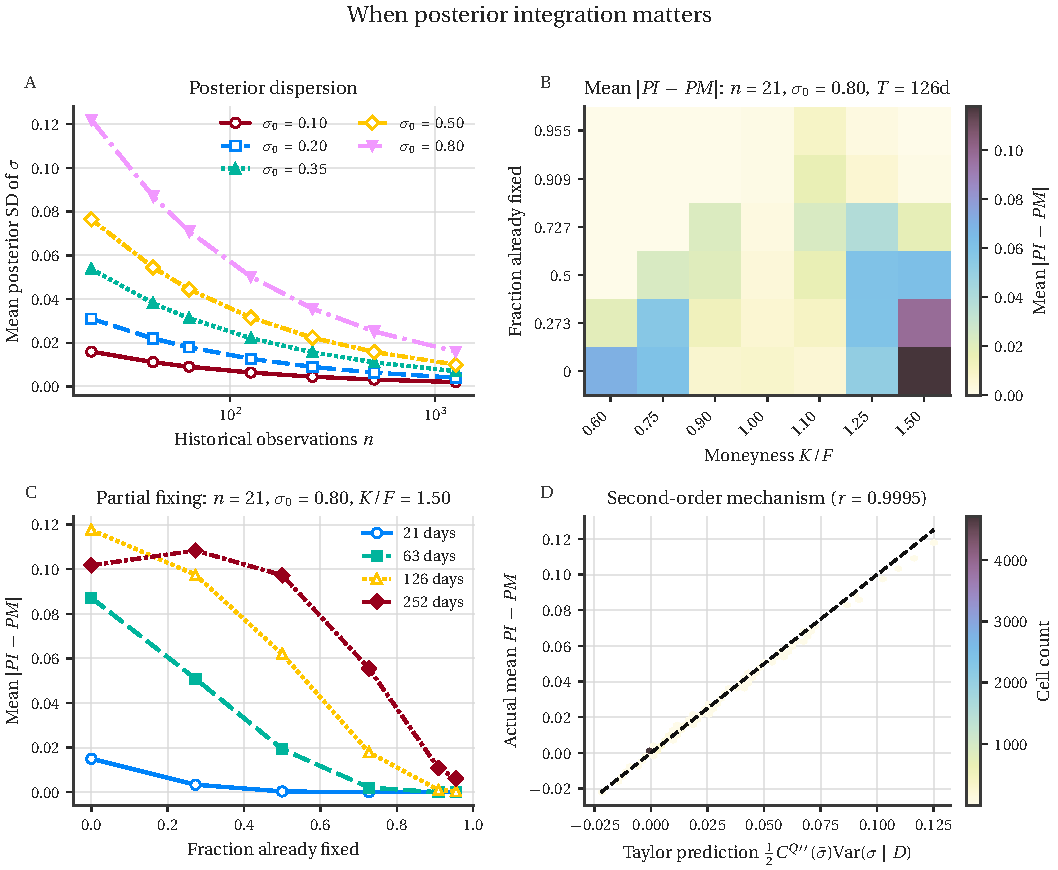
\includegraphics[width=\textwidth]{figures/publication/fig01_mechanism_map.pdf}
\caption{Posterior integration across synthetic WTI-like states. Panel A shows posterior dispersion against historical sample size. Panels B and C show how the absolute PI--PM difference varies with moneyness and the fraction of the averaging period already fixed. Panel D compares cell-level mean PI--PM differences with the corresponding second-order approximation in Equation~\eqref{eq:short_taylor}; the correlation is 0.9995. The color bar labeled \textit{Cell count} records how many synthetic scenario cells fall in each hexagonal bin of Panel D.}
\label{fig:short_mechanism}
\end{figure*}

\subsection{WTI point-price correction versus parameter uncertainty}

The October-2026 baseline contains 310 contract-date observations over 12 eligible valuation dates. Table~\ref{tab:short_october} reports the main Bayesian comparison. Posterior-integrated and posterior-mean plug-in prices have nearly identical market-pricing errors: RMSE is 0.5177 for PI and 0.5183 for PM. The mean absolute difference between the two prices is only 0.000745.

That near equality does not imply that uncertainty in the theoretical option value is negligible. The mean width of the central 95\% posterior interval for the model price is 0.2733, approximately 367 times the mean absolute PI--PM difference. The two quantities answer different questions. PI--PM measures how nonlinear averaging changes the posterior expectation of the option value; the interval width measures the dispersion of theoretical prices induced by uncertainty about volatility.

\begin{table}[t]
\centering
\caption{October-2026 WTI APO pricing and posterior price uncertainty. Pricing error is model price minus settlement price. All price quantities and errors are in U.S. dollars per barrel.}\label{tab:short_october}
\begin{tabular}{lrr}
\toprule
Quantity & $N$ & Value \\
\midrule
PI RMSE & 310 & 0.5177 \\
PM plug-in RMSE & 310 & 0.5183 \\
Mean $|PI-PM|$ & 310 & 0.000745 \\
Mean 95\% posterior price-interval width & 310 & 0.2733 \\
\bottomrule
\end{tabular}
\end{table}

The common pricing bias also points away from posterior integration as the main empirical margin. Both historical-volatility prices understate settlement values on average in the October baseline, and PI and PM differ by less than one tenth of a cent per barrel on average. A different volatility input therefore has much more room to affect pricing performance than a more exact integration of this relatively concentrated posterior.

\subsection{Historical versus option-implied volatility}

Table~\ref{tab:short_forward} reports the central out-of-sample comparison. On the same 2,381 contract-date observations, the long-window historical posterior-integrated benchmark has MAE 2.6187 and RMSE 3.4090. The best of the pre-specified rolling-window comparisons, based on the most recent 63 returns, has still larger errors, with MAE 4.5201 and RMSE 5.6465. The horizon-matched GARCH(1,1) benchmark produces MAE 2.6730 and RMSE 3.4441, close to the long-window historical benchmark.

By contrast, the previous-day APO implied-volatility smile has MAE 0.1075 and RMSE 0.1594. The expanding earlier-date smile produces similarly small errors, 0.1088 and 0.1725. The difference is present in every admitted expiry rather than being produced by one maturity. Valuation-date cluster bootstrap intervals for the error differences also remain well below zero across the seven expiries, as shown in Figure~\ref{fig:short_forward_bootstrap}.

\begin{table*}[t]
\centering
\caption{Historical-volatility and prior option-implied volatility benchmarks. Panel A uses the same 2,381 out-of-sample contract-date observations over 15 target dates. Panel B restricts the comparison to observations for which the same contract has a strictly prior implied volatility. Historical PI is the canonical Monte Carlo posterior-integrated price; scalar historical, GARCH, and implied-volatility inputs are repriced under the same Curran approximation. MAE and RMSE are in U.S. dollars per barrel.}\label{tab:short_forward}

\textit{Panel A: main out-of-sample comparison}\\[2pt]
\begin{tabular}{lrrrr}
\toprule
Volatility input & $N$ & Dates & MAE & RMSE\\
\midrule
Historical PI & 2,381 & 15 & 2.6187 & 3.4090\\
Rolling 63 returns & 2,381 & 15 & 4.5201 & 5.6465\\
Horizon-matched GARCH(1,1) & 2,381 & 15 & 2.6730 & 3.4441\\
Previous-day APO implied-volatility smile & 2,381 & 15 & 0.1075 & 0.1594\\
\bottomrule
\end{tabular}

\vspace{5pt}
\textit{Panel B: same-contract lagged-IV benchmark}\\[2pt]
\begin{tabular}{lrrrr}
\toprule
Volatility input & $N$ & Dates & MAE & RMSE\\
\midrule
Historical PI & 2,366 & 15 & 2.6279 & 3.4173\\
Same-contract lagged IV & 2,366 & 15 & 0.0992 & 0.1403\\
Previous-day fitted APO smile & 2,366 & 15 & 0.1074 & 0.1594\\
\bottomrule
\end{tabular}
\end{table*}

The historical comparisons address two natural alternatives. First, the difference is not reproduced by simply shortening the return window or by using an exponentially weighted historical estimate; the complete set of rolling-window and EWMA results is reported in Online Supplement Section S1 and Table S1. Second, allowing conditional heteroskedasticity and forecasting variance over the remaining fixing horizon does not materially close the pooled gap: GARCH remains near the long-window historical benchmark.

Panel B addresses a different alternative. On the exact common sample, carrying the same contract's latest prior implied volatility forward has lower pooled MAE and RMSE than fitting the previous-day smile. This is a descriptive ranking rather than evidence that lagged IV is generally superior to a fitted smile. Its role is to show that the large historical-versus-option-implied difference does not require a flexible cross-sectional implied-volatility function.

\begin{figure*}[t]
\centering
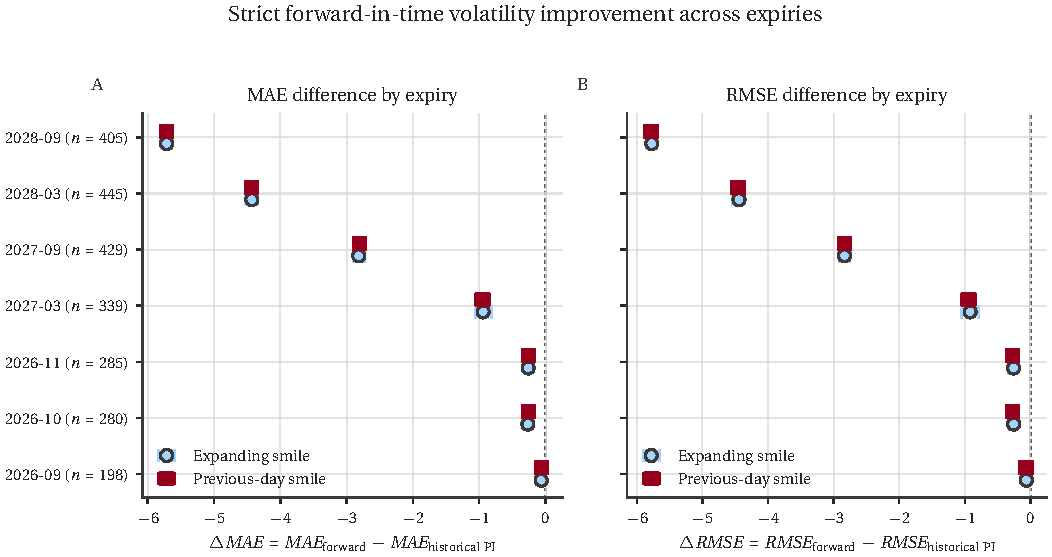
\includegraphics[width=\textwidth]{figures/publication/fig03_forward_q_cluster_bootstrap.pdf}
\caption{Out-of-sample pricing-error differences by APO expiry. Points compare the earlier-date APO implied-volatility specifications with the historical posterior-integrated benchmark; negative values indicate lower error for the implied-volatility specification. Horizontal bars are 95\% percentile intervals from valuation-date cluster bootstrap resampling. All implied-volatility inputs are estimated only from dates earlier than the target date.}
\label{fig:short_forward_bootstrap}
\end{figure*}

The economic interpretation should remain conditional on the model. Historical volatility and option-implied volatility are not two estimators of an identical observable object. The latter can incorporate risk premia and can also compensate for omitted stochastic volatility, jumps, futures-curve dynamics, and market-marking effects. The out-of-sample result therefore establishes a difference in pricing information under the maintained model, not a structural decomposition of the physical and risk-neutral volatility processes.

\subsection{Cross-instrument validation using vanilla-WTI options}

The independent vanilla-WTI experiment moves the implied-volatility source outside the APO market. Table~\ref{tab:short_lo} reports the exact common sample of 253 October-2026 APO contract-dates over 10 valuation dates. Historical-volatility posterior integration has MAE 0.4464 and RMSE 0.5562. A previous-day vanilla-WTI implied-volatility specification based on LO options lowers these errors to 0.1559 and 0.2599. The corresponding previous-day APO implied-volatility smile has MAE 0.1676 and RMSE 0.2686.

\begin{table}[t]
\centering
\caption{Cross-instrument validation on 253 October-2026 APO contract-dates within observed prior LO moneyness support. Historical PI is the canonical Monte Carlo posterior-integrated price; the vanilla-WTI and APO implied-volatility inputs are repriced with the deterministic Curran approximation. All implied-volatility inputs use only earlier-date option information. MAE and RMSE are in U.S. dollars per barrel.}\label{tab:short_lo}
\begin{tabular}{lrr}
\toprule
Volatility input & MAE & RMSE\\
\midrule
Historical PI & 0.4464 & 0.5562\\
Previous-day vanilla-WTI IV & 0.1559 & 0.2599\\
Previous-day APO IV & 0.1676 & 0.2686\\
\bottomrule
\end{tabular}
\end{table}

Valuation-date cluster bootstrap intervals preserve the improvement of the external LO specification relative to historical volatility. The external and APO-implied results are much closer to one another, and their difference is not uniformly distinguishable across MAE and RMSE. The relevant conclusion is therefore not that LO is superior to APO-implied volatility. It is that the pricing improvement associated with prior option-implied volatility persists when the information is obtained from another WTI option family.

Taken together, the results separate the two empirical margins. Posterior integration can matter when posterior variance meets option-price curvature, and the synthetic experiment identifies those states clearly. In the observed WTI sample, however, the PI--PM point-price effect is small. The substantially larger empirical difference comes from the volatility information supplied to the pricing model.

\section{Robustness and interpretation}\label{sec:short_robustness}

The main results are accompanied by a broader set of diagnostics reported in the online supplement. Complete rolling-window and EWMA comparisons are in Section S1; numerical accuracy and posterior calibration are in Section S2; liquidity restrictions are in Section S3; and LO scalar-transfer and tree-refinement diagnostics are in Section S4. These checks determine whether the three central findings depend on a particular historical specification, numerical method, or data construction, but they are not separate contributions.

First, changing the physical-measure specification does not materially alter the main pricing hierarchy. A standardized Student-\(t\) return model modestly changes the historical-volatility estimates but leaves the PI--PM difference small relative to the remaining model-to-market pricing error. Reconstructing the historical return series contract by contract from first-nearby CL settlements produces a posterior volatility estimate close to the continuous/front-month proxy. On the 2,381 out-of-sample observations, the reconstructed historical benchmark has MAE 2.6468 and RMSE 3.4451, compared with 2.6187 and 3.4090 for the baseline historical series.

Second, the near equality of PI and the posterior-mean plug-in price is not a numerical artifact. Difficult contracts are repriced with high-precision pseudo-random Monte Carlo, independently scrambled Sobol sequences, and Curran conditioning. These methods recover the PI--PM difference at a numerical scale well below the observed empirical gaps. Simulation-based calibration provides a separate check on posterior implementation. A posterior-RMS volatility,
\[
 \sigma_{\mathrm{RMS}}=\sqrt{\mathbb E[\sigma^2\mid\mathcal D]},
\]
also changes pooled pricing errors only slightly when compared with posterior mean volatility under the same Curran approximation. This reinforces the conclusion that the choice among nearby scalar summaries of the historical posterior is not the main empirical pricing margin; the detailed numerical and calibration results appear in Online Supplement Section S2 and Table S2.

Third, the external vanilla-WTI experiment is robust to the mapping from maturity-specific LO implied volatilities to the scalar volatility required by the maintained APO model. Replacing the primary fixing-count RMS mapping with a scalar chosen to match the variance of the unresolved arithmetic-average component changes pricing errors only slightly. An 80/160/320-step CRR refinement audit also shows practical stability of the LO implied-volatility inversion at the production 160-step choice. These are numerical stability checks, not claims of exact convergence or of a globally arbitrage-free fitted volatility surface; the alternative transfer and refinement results are reported in Online Supplement Section S4 and Table S4.

Liquidity and cross-sectional dependence remain important limitations. The main option panel contains many end-of-day settlements with zero reported volume, particularly at longer maturities. Restricting the forward comparison by positive volume or open interest preserves the large historical-versus-option-implied difference, but transaction-active observations become sparse within some individual expiries. Valuation-date cluster resampling addresses contemporaneous dependence across contracts, but the 15 APO target dates and 10 external-validation dates do not constitute long independent market histories. The liquidity-restricted results are summarized in Online Supplement Section S3 and Table S3.

The maintained one-factor model is deliberately restrictive. A richer commodity model could allow multiple futures-curve factors, stochastic volatility, jumps, stochastic convenience yield, or stochastic interest rates. Such extensions may reduce absolute pricing errors, but they would answer a different question. The present design keeps the pricing specification fixed to identify the relative importance of posterior integration and volatility information within one common framework.

Accordingly, the option-implied advantage should not be interpreted as a direct estimate of a variance risk premium or as evidence that a single structural risk-neutral volatility exists. Implied volatility in this exercise is the volatility required by the maintained pricing model to match observed option prices. It can absorb risk premia, omitted dynamics, liquidity effects, and settlement conventions. The empirical result is narrower and more defensible: prior option-implied volatility contains more useful information for the subsequent APO settlements in this sample than the historical-volatility benchmarks evaluated here.

\section{Conclusion}\label{sec:short_conclusion}

This paper separates two questions in Bayesian option pricing: whether parameter uncertainty materially changes the posterior mean option value, and whether the source of the volatility input materially changes out-of-sample pricing performance. The first question is governed locally by posterior variance and curvature of the option-pricing function. The synthetic experiment confirms this mechanism and shows that posterior integration can become economically relevant in weak-information, high-curvature states.

The observed WTI sample lies in a different region. Posterior-integrated and posterior-mean plug-in prices are almost identical, while the posterior distribution of model prices remains materially dispersed. A small PI--PM difference therefore does not imply little parameter uncertainty in the option value; it means that nonlinear averaging changes the posterior mean price very little in the observed states.

The larger empirical margin is the volatility information supplied to the pricing model. Prior option-implied volatility produces substantially lower out-of-sample pricing errors than the historical-volatility benchmarks evaluated here. The result is robust to recent-window, EWMA, and horizon-matched GARCH comparisons, does not require a flexible implied-volatility smile, and persists when the volatility input is obtained from a separate vanilla-WTI option market.

These findings are conditional on a small number of market dates and on the maintained one-factor pricing model. They do not identify a structural physical-versus-risk-neutral volatility wedge. Their narrower implication is that, for these WTI APOs, improving the volatility information is much more consequential for point pricing than integrating a relatively concentrated historical-volatility posterior more exactly.


\bmsection*{Data availability}
The WTI APO and CL histories used in the empirical application were obtained through a commercial Barchart subscription. The independent vanilla-WTI validation uses CME/NYMEX LO option and CL futures statistics accessed through Databento. Raw proprietary market-data files are not redistributed. The public repository provides code, query metadata, schemas, provenance records, diagnostics, hashes, and derived results consistent with the applicable data licenses.

\bmsection*{Code availability}
The research code is organized as the Python package \texttt{bayesian\_asian\_options}, with tests, deterministic experiment entry points, and committed derived results. The public repository is \url{https://github.com/heri-espino/Bayesian-Uncertainty-in-WTI-APOs}. The computational snapshot underlying this revision is Git commit \texttt{8d95e5313e7b764c0cb0e7f9ef06e54bcf5d75d7}.

\bmsection*{Conflict of interest}
The author declares no conflict of interest.

\bmsection*{Acknowledgments}
To be completed before submission.

\bibliography{references}

\end{document}
